\documentclass[a4paper]{article}

\usepackage[pdftex,
  hidelinks,
  pdfauthor={Dexter Chua},
  pdfsubject={Cambridge Maths Notes: Part IA - Dynamics and Relativity},
  pdftitle={Part IA - Dynamics and Relativity},
pdfkeywords={Cambridge Mathematics Maths Math IA Lent Dynamics and Relativity}]{hyperref}

% Imports
\ifx \nextra \undefined
  \usepackage[pdftex,
    hidelinks,
    pdfauthor={Dexter Chua},
    pdfsubject={Cambridge Maths Notes: Part \npart\ - \ncourse},
    pdftitle={Part \npart\ - \ncourse},
  pdfkeywords={Cambridge Mathematics Maths Math \npart\ \nterm\ \nyear\ \ncourse}]{hyperref}
  \title{Part \npart\ - \ncourse}
\else
  \usepackage[pdftex,
    hidelinks,
    pdfauthor={Dexter Chua},
    pdfsubject={Cambridge Maths Notes: Part \npart\ - \ncourse\ (\nextra)},
    pdftitle={Part \npart\ - \ncourse\ (\nextra)},
  pdfkeywords={Cambridge Mathematics Maths Math \npart\ \nterm\ \nyear\ \ncourse\ \nextra}]{hyperref}

  \title{Part \npart\ - \ncourse \\ {\Large \nextra}}
\fi

\author{Lectured by \nlecturer \\\small Notes taken by Dexter Chua}
\date{\nterm\ \nyear}

\usepackage{alltt}
\usepackage{amsfonts}
\usepackage{amsmath}
\usepackage{amssymb}
\usepackage{amsthm}
\usepackage{booktabs}
\usepackage{caption}
\usepackage{enumitem}
\usepackage{fancyhdr}
\usepackage{graphicx}
\usepackage{mathtools}
\usepackage{microtype}
\usepackage{multirow}
\usepackage{pdflscape}
\usepackage{pgfplots}
\usepackage{siunitx}
\usepackage{tabularx}
\usepackage{tikz}
\usepackage{tkz-euclide}
\usepackage[normalem]{ulem}
\usepackage[all]{xy}

\pgfplotsset{compat=1.12}

\pagestyle{fancyplain}
\lhead{\emph{\nouppercase{\leftmark}}}
\ifx \nextra \undefined
  \rhead{
    \ifnum\thepage=1
    \else
      \npart\ \ncourse
    \fi}
\else
  \rhead{
    \ifnum\thepage=1
    \else
      \npart\ \ncourse\ (\nextra)
    \fi}
\fi
\usetikzlibrary{arrows}
\usetikzlibrary{decorations.markings}
\usetikzlibrary{decorations.pathmorphing}
\usetikzlibrary{positioning}
\usetikzlibrary{fadings}
\usetikzlibrary{intersections}
\usetikzlibrary{cd}

\newcommand*{\Cdot}{\raisebox{-0.25ex}{\scalebox{1.5}{$\cdot$}}}
\newcommand {\pd}[2][ ]{
  \ifx #1 { }
    \frac{\partial}{\partial #2}
  \else
    \frac{\partial^{#1}}{\partial #2^{#1}}
  \fi
}

% Theorems
\theoremstyle{definition}
\newtheorem*{aim}{Aim}
\newtheorem*{axiom}{Axiom}
\newtheorem*{claim}{Claim}
\newtheorem*{cor}{Corollary}
\newtheorem*{defi}{Definition}
\newtheorem*{eg}{Example}
\newtheorem*{fact}{Fact}
\newtheorem*{law}{Law}
\newtheorem*{lemma}{Lemma}
\newtheorem*{notation}{Notation}
\newtheorem*{prop}{Proposition}
\newtheorem*{thm}{Theorem}

\renewcommand{\labelitemi}{--}
\renewcommand{\labelitemii}{$\circ$}
\renewcommand{\labelenumi}{(\roman{*})}

\let\stdsection\section
\renewcommand\section{\newpage\stdsection}

% Strike through
\def\st{\bgroup \ULdepth=-.55ex \ULset}

% Maths symbols
\newcommand{\bra}{\langle}
\newcommand{\ket}{\rangle}

\newcommand{\N}{\mathbb{N}}
\newcommand{\Z}{\mathbb{Z}}
\newcommand{\Q}{\mathbb{Q}}
\renewcommand{\H}{\mathbb{H}}
\newcommand{\R}{\mathbb{R}}
\newcommand{\C}{\mathbb{C}}
\newcommand{\Prob}{\mathbb{P}}
\renewcommand{\P}{\mathbb{P}}
\newcommand{\E}{\mathbb{E}}
\newcommand{\F}{\mathbb{F}}
\newcommand{\cU}{\mathcal{U}}
\newcommand{\RP}{\mathbb{RP}}
\newcommand{\CP}{\mathbb{CP}}

\newcommand{\ph}{\,\cdot\,}

\DeclareMathOperator{\sech}{sech}
\DeclareMathOperator{\cosech}{cosech}
\DeclareMathOperator{\cosec}{cosec}

\DeclareMathOperator{\covol}{covol}
\DeclareMathOperator{\vol}{vol}

\let\Im\relax
\let\Re\relax
\DeclareMathOperator{\Im}{Im}
\DeclareMathOperator{\Re}{Re}
\DeclareMathOperator{\im}{im}
\DeclareMathOperator{\image}{image}
\DeclareMathOperator{\Ann}{Ann}

\DeclareMathOperator*{\res}{res}
\DeclareMathOperator{\Res}{Res}
\DeclareMathOperator{\Ind}{Ind}

\DeclareMathOperator{\tr}{tr}
\DeclareMathOperator{\diag}{diag}
\DeclareMathOperator{\rank}{rank}
\DeclareMathOperator{\card}{card}
\DeclareMathOperator{\spn}{span}
\DeclareMathOperator{\adj}{adj}

\DeclareMathOperator{\erf}{erf}
\DeclareMathOperator{\erfc}{erfc}

\DeclareMathOperator{\ord}{ord}
\DeclareMathOperator{\Sym}{Sym}

\DeclareMathOperator{\sgn}{sgn}
\DeclareMathOperator{\orb}{orb}
\DeclareMathOperator{\stab}{stab}
\DeclareMathOperator{\ccl}{ccl}

\DeclareMathOperator{\lcm}{lcm}
\DeclareMathOperator{\hcf}{hcf}

\DeclareMathOperator{\Int}{Int}
\DeclareMathOperator{\id}{id}

\DeclareMathOperator{\betaD}{beta}
\DeclareMathOperator{\gammaD}{gamma}
\DeclareMathOperator{\Poisson}{Poisson}
\DeclareMathOperator{\binomial}{binomial}
\DeclareMathOperator{\multinomial}{multinomial}
\DeclareMathOperator{\Bernoulli}{Bernoulli}
\DeclareMathOperator{\like}{like}

\DeclareMathOperator{\var}{var}
\DeclareMathOperator{\cov}{cov}
\DeclareMathOperator{\bias}{bias}
\DeclareMathOperator{\mse}{mse}
\DeclareMathOperator{\corr}{corr}

\DeclareMathOperator{\otp}{otp}
\DeclareMathOperator{\dom}{dom}

\DeclareMathOperator{\Root}{Root}
\DeclareMathOperator{\supp}{supp}
\DeclareMathOperator{\rel}{rel}
\DeclareMathOperator{\Hom}{Hom}
\DeclareMathOperator{\Aut}{Aut}
\DeclareMathOperator{\Gal}{Gal}
\DeclareMathOperator{\Mat}{Mat}
\DeclareMathOperator{\End}{End}
\DeclareMathOperator{\Char}{char}
\DeclareMathOperator{\ev}{ev}
\DeclareMathOperator{\St}{St}
\DeclareMathOperator{\Lk}{Lk}
\DeclareMathOperator{\disc}{disc}
\DeclareMathOperator{\Isom}{Isom}
\DeclareMathOperator{\length}{length}
\DeclareMathOperator{\energy}{energy}
\DeclareMathOperator{\area}{area}
\DeclareMathOperator{\Syl}{Syl}
\DeclareMathOperator{\cl}{cl}
\DeclareMathOperator{\fix}{fix}

\newcommand{\GL}{\mathrm{GL}}
\newcommand{\SL}{\mathrm{SL}}
\newcommand{\PGL}{\mathrm{PGL}}
\newcommand{\PSL}{\mathrm{PSL}}
\newcommand{\PSU}{\mathrm{PSU}}
\newcommand{\Or}{\mathrm{O}}
\newcommand{\SO}{\mathrm{SO}}
\newcommand{\U}{\mathrm{U}}
\newcommand{\SU}{\mathrm{SU}}

\renewcommand{\d}{\mathrm{d}}
\newcommand{\D}{\mathrm{D}}

\tikzset{->/.style = {decoration={markings,
                                  mark=at position 1 with {\arrow[scale=2]{latex'}}},
                      postaction={decorate}}}
\tikzset{<-/.style = {decoration={markings,
                                  mark=at position 0 with {\arrowreversed[scale=2]{latex'}}},
                      postaction={decorate}}}
\tikzset{<->/.style = {decoration={markings,
                                   mark=at position 0 with {\arrowreversed[scale=2]{latex'}},
                                   mark=at position 1 with {\arrow[scale=2]{latex'}}},
                       postaction={decorate}}}
\tikzset{->-/.style = {decoration={markings,
                                   mark=at position #1 with {\arrow[scale=2]{latex'}}},
                       postaction={decorate}}}
\tikzset{-<-/.style = {decoration={markings,
                                   mark=at position #1 with {\arrowreversed[scale=2]{latex'}}},
                       postaction={decorate}}}

\tikzset{circ/.style = {fill, circle, inner sep = 0, minimum size = 3}}
\tikzset{mstate/.style={circle, draw, blue, text=black, minimum width=0.7cm}}

\definecolor{mblue}{rgb}{0.2, 0.3, 0.8}
\definecolor{morange}{rgb}{1, 0.5, 0}
\definecolor{mgreen}{rgb}{0.1, 0.4, 0.2}
\definecolor{mred}{rgb}{0.5, 0, 0}

\def\drawcirculararc(#1,#2)(#3,#4)(#5,#6){%
    \pgfmathsetmacro\cA{(#1*#1+#2*#2-#3*#3-#4*#4)/2}%
    \pgfmathsetmacro\cB{(#1*#1+#2*#2-#5*#5-#6*#6)/2}%
    \pgfmathsetmacro\cy{(\cB*(#1-#3)-\cA*(#1-#5))/%
                        ((#2-#6)*(#1-#3)-(#2-#4)*(#1-#5))}%
    \pgfmathsetmacro\cx{(\cA-\cy*(#2-#4))/(#1-#3)}%
    \pgfmathsetmacro\cr{sqrt((#1-\cx)*(#1-\cx)+(#2-\cy)*(#2-\cy))}%
    \pgfmathsetmacro\cA{atan2(#2-\cy,#1-\cx)}%
    \pgfmathsetmacro\cB{atan2(#6-\cy,#5-\cx)}%
    \pgfmathparse{\cB<\cA}%
    \ifnum\pgfmathresult=1
        \pgfmathsetmacro\cB{\cB+360}%
    \fi
    \draw (#1,#2) arc (\cA:\cB:\cr);%
}
\newcommand\getCoord[3]{\newdimen{#1}\newdimen{#2}\pgfextractx{#1}{\pgfpointanchor{#3}{center}}\pgfextracty{#2}{\pgfpointanchor{#3}{center}}}

\def\Xint#1{\mathchoice
   {\XXint\displaystyle\textstyle{#1}}%
   {\XXint\textstyle\scriptstyle{#1}}%
   {\XXint\scriptstyle\scriptscriptstyle{#1}}%
   {\XXint\scriptscriptstyle\scriptscriptstyle{#1}}%
   \!\int}
\def\XXint#1#2#3{{\setbox0=\hbox{$#1{#2#3}{\int}$}
     \vcenter{\hbox{$#2#3$}}\kern-.5\wd0}}
\def\ddashint{\Xint=}
\def\dashint{\Xint-}



\title{Part IA - Dynamics and Relativity}
\author{Lectured by G. I. Ogilvie}
\date{Lent 2015}

\begin{document}
\maketitle
{\small
\noindent\textbf{Basic concepts}\\
Space and time, frames of reference, Galilean transformations. Newton's laws. Dimensional analysis.  Examples of forces, including gravity, friction and Lorentz.\hspace*{\fill} [4]

\vspace{10pt}
\noindent\textbf{Newtonian dynamics of a single particle}\\
Equation of motion in Cartesian and plane polar coordinates. Work, conservative forces and potential energy, motion and the shape of the potential energy function; stable equilibria and small oscillations; effect of damping.

\vspace{5pt}
\noindent Angular velocity, angular momentum, torque.

\vspace{5pt}
\noindent Orbits: the $u(\theta)$ equation; escape velocity; Kepler's laws; stability of orbits; motion in a repulsive potential (Rutherford scattering). Rotating frames: centrifugal and coriolis forces. *Brief discussion of Foucault pendulum.*\hspace*{\fill} [8]

\vspace{10pt}
\noindent\textbf{Newtonian dynamics of systems of particles}\\
Momentum, angular momentum, energy. Motion relative to the centre of mass; the two body problem.  Variable mass problems; the rocket equation.\hspace*{\fill} [2]

\vspace{10pt}
\noindent\textbf{Rigid bodies}\\
Moments of inertia, angular momentum and energy of a rigid body. Parallel axes theorem. Simple examples of motion involving both rotation and translation (e.g. rolling).\hspace*{\fill} [3]

\vspace{10pt}
\noindent\textbf{Special relativity}\\
The principle of relativity. Relativity and simultaneity. The invariant interval. Lorentz transformations in $(1 + 1)$-dimensional spacetime. Time dilation and length contraction. The Minkowski metric for $(1 + 1)$-dimensional spacetime. Lorentz transformations in $(3 + 1)$ dimensions. 4-vectors and Lorentz invariants. Proper time. 4-velocity and 4-momentum. Conservation of 4-momentum in particle decay. Collisions. The Newtonian limit.\hspace*{\fill} [7]}

\tableofcontents
\section{Newtonian dynamics of particles}
We start with a few basic definitions:
\begin{defi}[Particle]
  An \emph{particle} is an object of insignificant size. It can be regarded as a point. It has a \emph{mass} $m > 0$, and \emph{electric charge} $q$.

  Its position at time $t$ is described by its \emph{position vector}, $\mathbf{r}(t)$ or $\mathbf{x}(t)$ with respect to an origin $O$.
\end{defi}

\begin{defi}[Frame of reference]
  A \emph{frame of reference} is choice of coordinate axes for $\mathbf{r}$. The axes may be fixed, moving, or accelerating relative to another frame.

  With a frame of reference, we can write $\mathbf{r}$ in cartesian coordinates as $(x, y, z)$
\end{defi}

\begin{defi}[Velocity]
  The \emph{velocity} of the particle is
  \[
    \mathbf{v} = \dot{\mathbf{r}} = \frac{\d \mathbf{r}}{\d t}.
  \]
  and is tangent to the path or trajectory.
\end{defi}

\begin{defi}[Acceleration]
  The \emph{acceleration} of the particle is
  \[
    \mathbf{a} = \dot{\mathbf{v}} = \ddot{\mathbf{r}} = \frac{\d^2 \mathbf{r}}{d t^2}.
  \]
\end{defi}

\begin{defi}[Momentum]
  The \emph{momentum} of a particle is
  \[
    \mathbf{p} = m\mathbf{v} = m\dot{\mathbf{r}}.
  \]
  $m$ is the \emph{inertial mass} of the particle, and measures its reluctance to accelerate (c.f. Newton's Second Law)
\end{defi}

\subsection{Newton's laws of motion}
We begin by stating Newton's three laws of motion:
\begin{law}[Newton's First Law of Motion]
  A body remains at rest, or moves uniformly in a straight line, unless acted on by a force. (This is in fact Galileo's Law of Inertia)
\end{law}

\begin{law}[Newton's Second Law of Motion]
   The rate of change of momentum of a body is equal to the force acting on it (in both magnitude and direction).
\end{law}

\begin{law}[Newton's Third Law of Motion]
  To every action there is an equal and opposite reaction: the forces of two bodies on each other are equal and in opposite directions.
\end{law}
The first law might seem redundant given the second if interpreted literally. Therefore, we should be interpreting it in the different way:

Note that the first law isn't always true. Take yourself as a frame of reference. When you move around your room, things will seem like they are moving around (relative to you). When you sit down, they stop moving. However, on second thought, this is because you, the frame of reference, is accelerating, not the objects. The first law only holds in frames that are themselves not accelerating. We call these \emph{inertial frames}.
\begin{defi}[Inertial frames]
  \emph{Inertial frames} are frames of references in which the frames themselves are not accelerating. Newton's Laws only hold in inertial frames.
\end{defi}
The we can take the first law to assert that inertial frames exists. Even though the Earth itself is rotating and orbiting the sun, for most purposes, any fixed place on the Earth counts as an inertial frame.

\subsection{Galilean transformations}
Inertial frames aren't unique. If $S$ is an inertial frame, then any other frame $S'$ in uniform motion relative to $S$ is also inertial:
\begin{center}
  \begin{tikzpicture}
    \node at (0, 1.5) [left] {$S$};
    \node at (4, 1.5) [left] {$S'$};
    \draw [->] (0, 0) -- (0, 3) node [above] {$y$};
    \draw [->] (0, 0) -- (3, 0) node [right] {$x$};
    \draw [->] (4, 0) -- (4, 3) node [above] {$y'$};
    \draw [->] (4, 0) -- (7, 0) node [right] {$x'$};
    \draw [->] (4, 1.5) -- (4.5, 1.5) node [right] {$\mathbf{v}$};
  \end{tikzpicture}
\end{center}

Assuming the frames coincide at $t = 0$, then
\begin{align*}
  x' &= x - vt\\
  y' &= y\\
  z' &= z\\
  t' &= t
\end{align*}

Generally, the position vector transforms as
\[
  \mathbf{r}' = \mathbf{r} - \mathbf{v}t,
\]
where $\mathbf{v}$ is the (constant) velocity of $S'$ relative to $S$. The velocity and acceleration transform as follows:
\begin{align*}
  \dot{\mathbf{r}}' &= \dot{\mathbf{r}} - \mathbf{v}\\
  \ddot{\mathbf{r}}' &= \ddot{\mathbf{r}}\\
\end{align*}

\begin{defi}[Galilean boost]
  A Galilean boost is a change in frame of reference by
  \begin{align*}
    \mathbf{r}' &= \mathbf{r} - \mathbf{v}t\\
    t' &= t
  \end{align*}
  for a fixed, constant $\mathbf{v}$.
\end{defi}

In addition to Galilean boosts, we can construct new inertial frames by applying (any combination of) the following:
\begin{itemize}
  \item Translations of space:
    \[
      \mathbf{r}' = \mathbf{r} - \mathbf{r}_0
    \]
  \item Translations of time:
    \[
      t' = t - t_0
    \]
  \item Rotation (and reflection):
    \[
      \mathbf{r}' = R\mathbf{r}
    \]
    with $R\in O(3)$.
\end{itemize}
These transformations together generate the Galilean group.

\begin{law}[Galilean relativity]
  The \emph{principle of relativity} asserts that the laws of physics are the same in inertial frames.
\end{law}

This implies that physical processes work the same
\begin{itemize}
  \item at every point of space
  \item at all times
  \item in whichever direction we face
  \item at whatever constant velocity we travel.
\end{itemize}

In other words, the equations of Newtonian physics must have \emph{Galilean invariance}.

Since the laws of physics are the same regardless of your velocity, velocity must be a \emph{relative concept}, and there is no such thing as an ``absolute velocity'' that all inertial frames agree on.

However, all inertial frames must agree on whether you are accelerating or not (even though they need not agree on the direction of acceleration since you can rotate your frame). So acceleration is an \emph{absolute} concept.

\subsection{Newton's Second Law}
\begin{law}
  The \emph{equation of motion} for a particle subject to a force $F$ is
  \[
    \frac{\d \mathbf{p}}{\d t} = \mathbf{F},
  \]
  where $\mathbf{p} = m\mathbf{v} = m\ddot{\mathbf{r}}$ is the (linear) momentum of the particle. We say $m$ is the (inertial) mass of the particle, which is a measure of its reluctance to accelerate.
\end{law}

Usually, $m$ is constant. Then
\[
  \mathbf{F} = m\mathbf{a} = m\ddot{\mathbf{r}}.
\]


If $\mathbf{F}$ is specified as a function of $\mathbf{r}, \dot{\mathbf{r}}$ and $t$, then we have a second-order ordinary differential equation for $\mathbf{r}$.

To determine the solution, we need to specify the initial values of $\mathbf{r}$ and $\dot{\mathbf{r}}$, i.e. the initial position and velocity. The trajectory of the particle is then uniquely determined for all future (and past) times.

\section{Dimensional Analysis}
\begin{center}
  \includegraphics[width=250pt]{images/xkcd_dimensional_analysis.png}\\
  xkcd (Randall Munroe) CC-BY-NC 2.5
\end{center}
Physical quantities are not pure numbers, but have \emph{dimensions}. In any equation, the dimensions have to be consistent.

For many problems in dynamics, three basic dimensions are sufficient:
\begin{itemize}
  \item length, $L$
  \item mass, $M$
  \item time, $T$
\end{itemize}

The dimensions of a physical quantity $X$, denoted as $[X]$ are expressible uniquely in terms of $L$, $M$ and $T$, e.g.
\begin{itemize}
  \item $[\text{area}] = L^2$
  \item $[\text{density}] = L^{-3} M$
  \item $[\text{velocity}] = LT^{-1}$
  \item $[\text{acceleration}] = LT^{-2}$
  \item $[\text{force}] = LMT^{-2}$ since the dimensions must satisfy the equation $F = ma$.
  \item $[\text{energy}] = L^2MT^{-2}$, e.g. consider $E = mv^2/2$.
\end{itemize}

Physical constants also have dimensions, e.g. $[G] = L^3M^{-1}T^{-2}$ by $F = GMm/r^2$.

We can only take sums and products of terms that have dimensions, and if we sum two terms, they must have the same dimension. More complicated functions of dimensional quantities are not allowed, e.g. $e^{x}$ makes no sense if $x$ has a dimension, since
\[
  e^x = 1 + x + \frac{1}{2}x^2 + \cdots
\]
and if $x$ had a dimension, we would be summing up terms of different dimensions.

\subsection{Units}
A \emph{unit} is a convenient standard physical quantity. In the SI system, there are base units corresponding to the basics dimensions. The three we need are 
\begin{itemize}
  \item meter (m) for length
  \item kilogram (kg) for mass
  \item second (s) for time
\end{itemize}
A physical quantity can be expressed as a pure number times a unit with the correct dimensions, e.g.
\[
  G = \SI{6.67e-11}{\meter\cubed\per\kilogram\per\second\squared}.
\]
It is important to realize that SI units are chosen arbitrarily for historical reasons only. The equation of physics must work in any consistent system of units. This is captured by the fact that physical equations must be dimensionally consistent.

\subsection{Scaling}
Suppose we believe that a physical quantity $Y$ depends on $3$ other physical quantities $X_1, X_2, X_3$, i.e. $Y = Y(X_1, X_2, X_3)$. Let their dimensions be as follows:
\begin{itemize}
  \item $[Y] = L^aM^bT^c$
  \item $[X_i] = L^{a_i}M^{b_i}T^{c_i}$
\end{itemize}
Suppose further that we know that the relationship is a power law, i.e. 
\[
  Y = CX_1^{p_1}X_2^{p_2}X_3^{p_3},
\]
where $C$ is a dimensionless constant (i.e. pure number). Since the dimensions must work out, we know that
\begin{align*}
  a &= p_1a_1 + p_2a_2 + p_3a_3\\
  b &= p_1b_1 + p_2b_2 + p_3b_3\\
  c &= p_1c_1 + p_2c_2 + p_3c_3
\end{align*}
for which there is a unique solution provided that the dimensions of $X_1, X_2$ and $X_3$ are independent.

Note that if $X_i$ are not independent, e.g. $X_1^2X_2$ is dimensionless, then our law can involve more complicated terms such as $\exp (X_1^2 X_2)$ since the argument to $\exp$ is dimensionless.

In general, if the dimensions of $X_i$ are not independent, order them so that the independent terms $[X_1], [X_2], [X_3]$ are at the front. For each of the remaining variables, form a dimensionless quantity $\lambda_i = X_iX_1^{q_1}X_2^{q_2}X_3^{q_3}$.
Then the relationship must be of the form
\[
  Y = f(\lambda_4, \lambda_5, \cdots) X_1^{p_1}X_2^{p_2}X_3^{p_3}.
\]
where $f$ is a dimensionless function of the dimensionless variables.

Formally, we have the \emph{Buckingham's Pi theorem}.

\begin{eg}[Simple pendulum]\leavevmode
  \begin{center}
    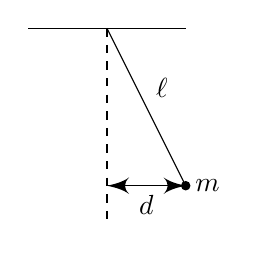
\begin{tikzpicture}
      \draw (-1, 0) -- (1, 0);
      \draw (0, 0) -- (1, -2) node [right] {$m$} node [draw, fill, circle, inner sep = 0, minimum size = 3] {} node [pos = 0.5, anchor = south west] {$\ell$};
      \draw [dashed] (0, 0) -- (0, -2.5);
      \draw [->] (0, -2) -- (1, -2) node [below, pos = 0.5] {$d$};
      \draw [->] (1, -2) -- (0, -2);
    \end{tikzpicture}
  \end{center}
  We want to find the period $P$. We know that $P$ could depend on 
  \begin{itemize}
    \item mass $m$: $[m] = M$
    \item length $\ell$: $[\ell] = L$
    \item gravity $g$: $[g] = LT^{-2}$
    \item initial displacement $d$: $[d] = L$
  \end{itemize}
  and of course $[P] = T$.

  We observe that $m, \ell, g$ have independent dimensions, and with the fourth, we can form the dimensionless group $d/\ell$. So the relationship must be of the form
  \[
    P = f\left(\frac{d}{l}\right) m^{p_1}\ell^{p_2}g^{p_3},
  \]
  where $f$ is a dimensionless function. For the dimensions to balance,
  \[
    T = M^{p_1}L^{p_2}L^{p_3}T^{-2p_3}.
  \]
  So $p_1 = 0, p_2 = -p_3 = 1/2$. Then
  \[
    P = f\left(\frac{d}{\ell}\right) \sqrt{\frac{\ell}{g}}.
  \]

  While we cannot find the exact formula, if $\ell$ is quadrupled and $d$ is also quadrupled, the $P$ will double. 
\end{eg}

\section{Forces}
\subsection{Force and potential energy in one dimension}
Consider a particle of mass $m$ moving in a straight line with position $x(t)$. Suppose $F = F(x)$, i.e. depends on position only. We define the potential energy as follows:
\begin{defi}[Potential energy]
  Given a force field $F = F(x)$, we define the \emph{potential energy} to be a function $V(x)$ such that
  \[
    F = -\frac{\d V}{\d x}.
  \]
  or
  \[
    V = -\int F \;\d x.
  \]
  $V$ includes an arbitrary additive constant.
\end{defi}

The equation of motion is then
\[
  m\ddot{x} = -\frac{\d V}{\d x}.\tag{*}
\]

\begin{prop}
  Suppose the equation of a particle satisfies
  \[
    m\ddot{x} = -\frac{\d V}{\d x}.\tag{*}
  \]
  Then the total energy
  \[
    E = T + V = \frac{1}{2} m\dot{x}^2 + V(x)
  \]
  is conserved, i.e. $\dot{E} = 0$.
\end{prop}

\begin{proof}
  \begin{align*}
    \frac{\d E}{\d t} &= m\dot{x}\ddot{x} + \frac{\d V}{\d x}\dot{x}\\
    &= \dot{x}\left(m\ddot{x} + \frac{\d V}{\d x}\right)\\
    &= 0
  \end{align*}
\end{proof}

\begin{eg}
  Consider the harmonic oscillator
  \[
    V = \frac{1}{2} kx^2.
  \]
  Then the equation of motion satisfy
  \[
    m\ddot{x} = -kx.
  \]
  This is the case of, say, Hooke's Law for a spring. But in general, small perturbations near potential wells are also harmonic oscillators.

  The general solution of this is
  \[
    x(t) = A\cos (\omega t) + B\sin (\omega t)
  \]
  with $\omega = \sqrt{k/m}$.

  $A$ and $B$ are arbitrary constants, and are related to the initial position and velocity by $x(0) = A, \dot{x}(0) = \omega B$.
\end{eg}

For a general potential energy $V(x)$, conservation of energy allows us to solve the problem formally:
\[
  E = \frac{1}{2}m\dot{x}^2 + V(x)
\]
Since $E$ is a constant, from this equation, we have
\begin{align*}
  \frac{\d x}{\d t} &= \pm \sqrt{\frac{2}{m}(E - V(x))}\\
  \pm \int \frac{\d x}{\sqrt{\frac{2}{m}(E - V(x))}} &= t - t_0
\end{align*}
To find $x(t)$, we need to do the integral, we need to do the integral and then solve for $x$ - not usually possible by analytical methods, but possible by numerical methods.

\subsection{Motion in a potential}
The graph of the potential energy $V(x)$ gives us a qualitative understanding of the dynamics, e.g. is the particle trapped or can it escape to infinity?

\begin{eg}
  Consider $V(x) = m(x^3 - 3x)$. Note that this can be dimensionally consistent even though we add up $x^3$ and $-3x$ if ``3'' has dimensions $L^2$.

  We plot this as follows:
  \begin{center}
    \begin{tikzpicture}
      \draw [->] (-3, 0) -- (3, 0) node [right] {$x$};
      \draw [domain=-2.2:2.2, samples=50] plot (\x, {0.5*(\x*\x*\x - 3*\x)});
      \draw [->] (0, -2) -- (0, 2) node [above] {$M$};
      \node [anchor = north east] {$O$};
      \draw (1, 0) -- (1, -0.1) node [below] {$1$};
      \draw (2, 0) -- (2, -0.1) node [below] {$2$};
      \draw (-1, 0) -- (-1, -0.1) node [below] {$-1$};
      \draw (-2, 0) -- (-2, -0.1) node [below] {$-2$};
    \end{tikzpicture}
  \end{center}

  Suppose we release the particle from rest at $x = x_0$. Then $E = V(x_0)$. We can consider the different cases:
  \begin{itemize}
    \item $x_0 = \pm 1$: Particle stays there for all $t$.
    \item $-1 < x_0 < 2$: Particle oscillates back and forth in potential well
    \item $x_0 < -1$: Particle falls to $x = -\infty$.
    \item $x_0 > 2$: Particle overshoots well and continues to $x = -\infty$.
    \item $x_0 = 2$: Special case: 
  \end{itemize}
\end{eg}
\end{document}

